%!TEX root=masterproef.tex

\subsection{Raamwerken voor detectie}
\label{subsection:frameworks}

Naast het onderzoek naar de verschillende autonome detectiealgoritmen, zijn er
ook onderzoekers actief op zoek naar manieren om meer holistische oplossingen
te bouwen die eerder het probleem als een geheel beschouwen in plaats van de
som van kleine, losse delen. In deze sectie bekijken we een aantal van deze
voorgestelde raamwerken.

\subsubsection*{Di-Sec}
\label{subsubsection:di-sec}

In \citep{valero2012di} komen de auteurs tot dezelfde conclusie als wij hier
reeds enkele malen hebben aangehaald: er wordt veel gekeken naar
detailoplossingen, maar zelden wordt een algemene oplossing voorgesteld voor de
typische situatie van DSN. De auteurs zijn het verder eveneens eens met de
stelling dat het belangrijk is om te leren van deze detailoplossingen om een
eventueel raamwerk af te stemmen op deze oplossingen en gebruikt te maken van
de goede eigenschappen ervan bij de implementatie van het eigenlijke raamwerk.

De auteurs gaan er in hun redenering van uit dat gegeven de eigenheid van het
draadloze medium, veel aanvallen zich inderdaad richten op deze
communicatiekanalen. Ze defini\"eren daarom een eerste component, COMM, die
zich toespitst op de communicatie en waarlangs alle gegevens passeren die
verstuurd en/of ontvangen worden. Daarnaast zijn er nog drie bijkomende
componenten: M-Core, de centrale controle module, Sense, de sensor module en de
DDMs, de detectie en verdedigingsmodules. Deze laatste zijn aanvalspecifieke
modules die ingevoegd kunnen worden in het raamwerk. Figuur
\ref{fig:di-sec-architecture} geeft een overzicht van de architectuur van
Di-Sec.

\begin{figure}[ht]
  \centering
  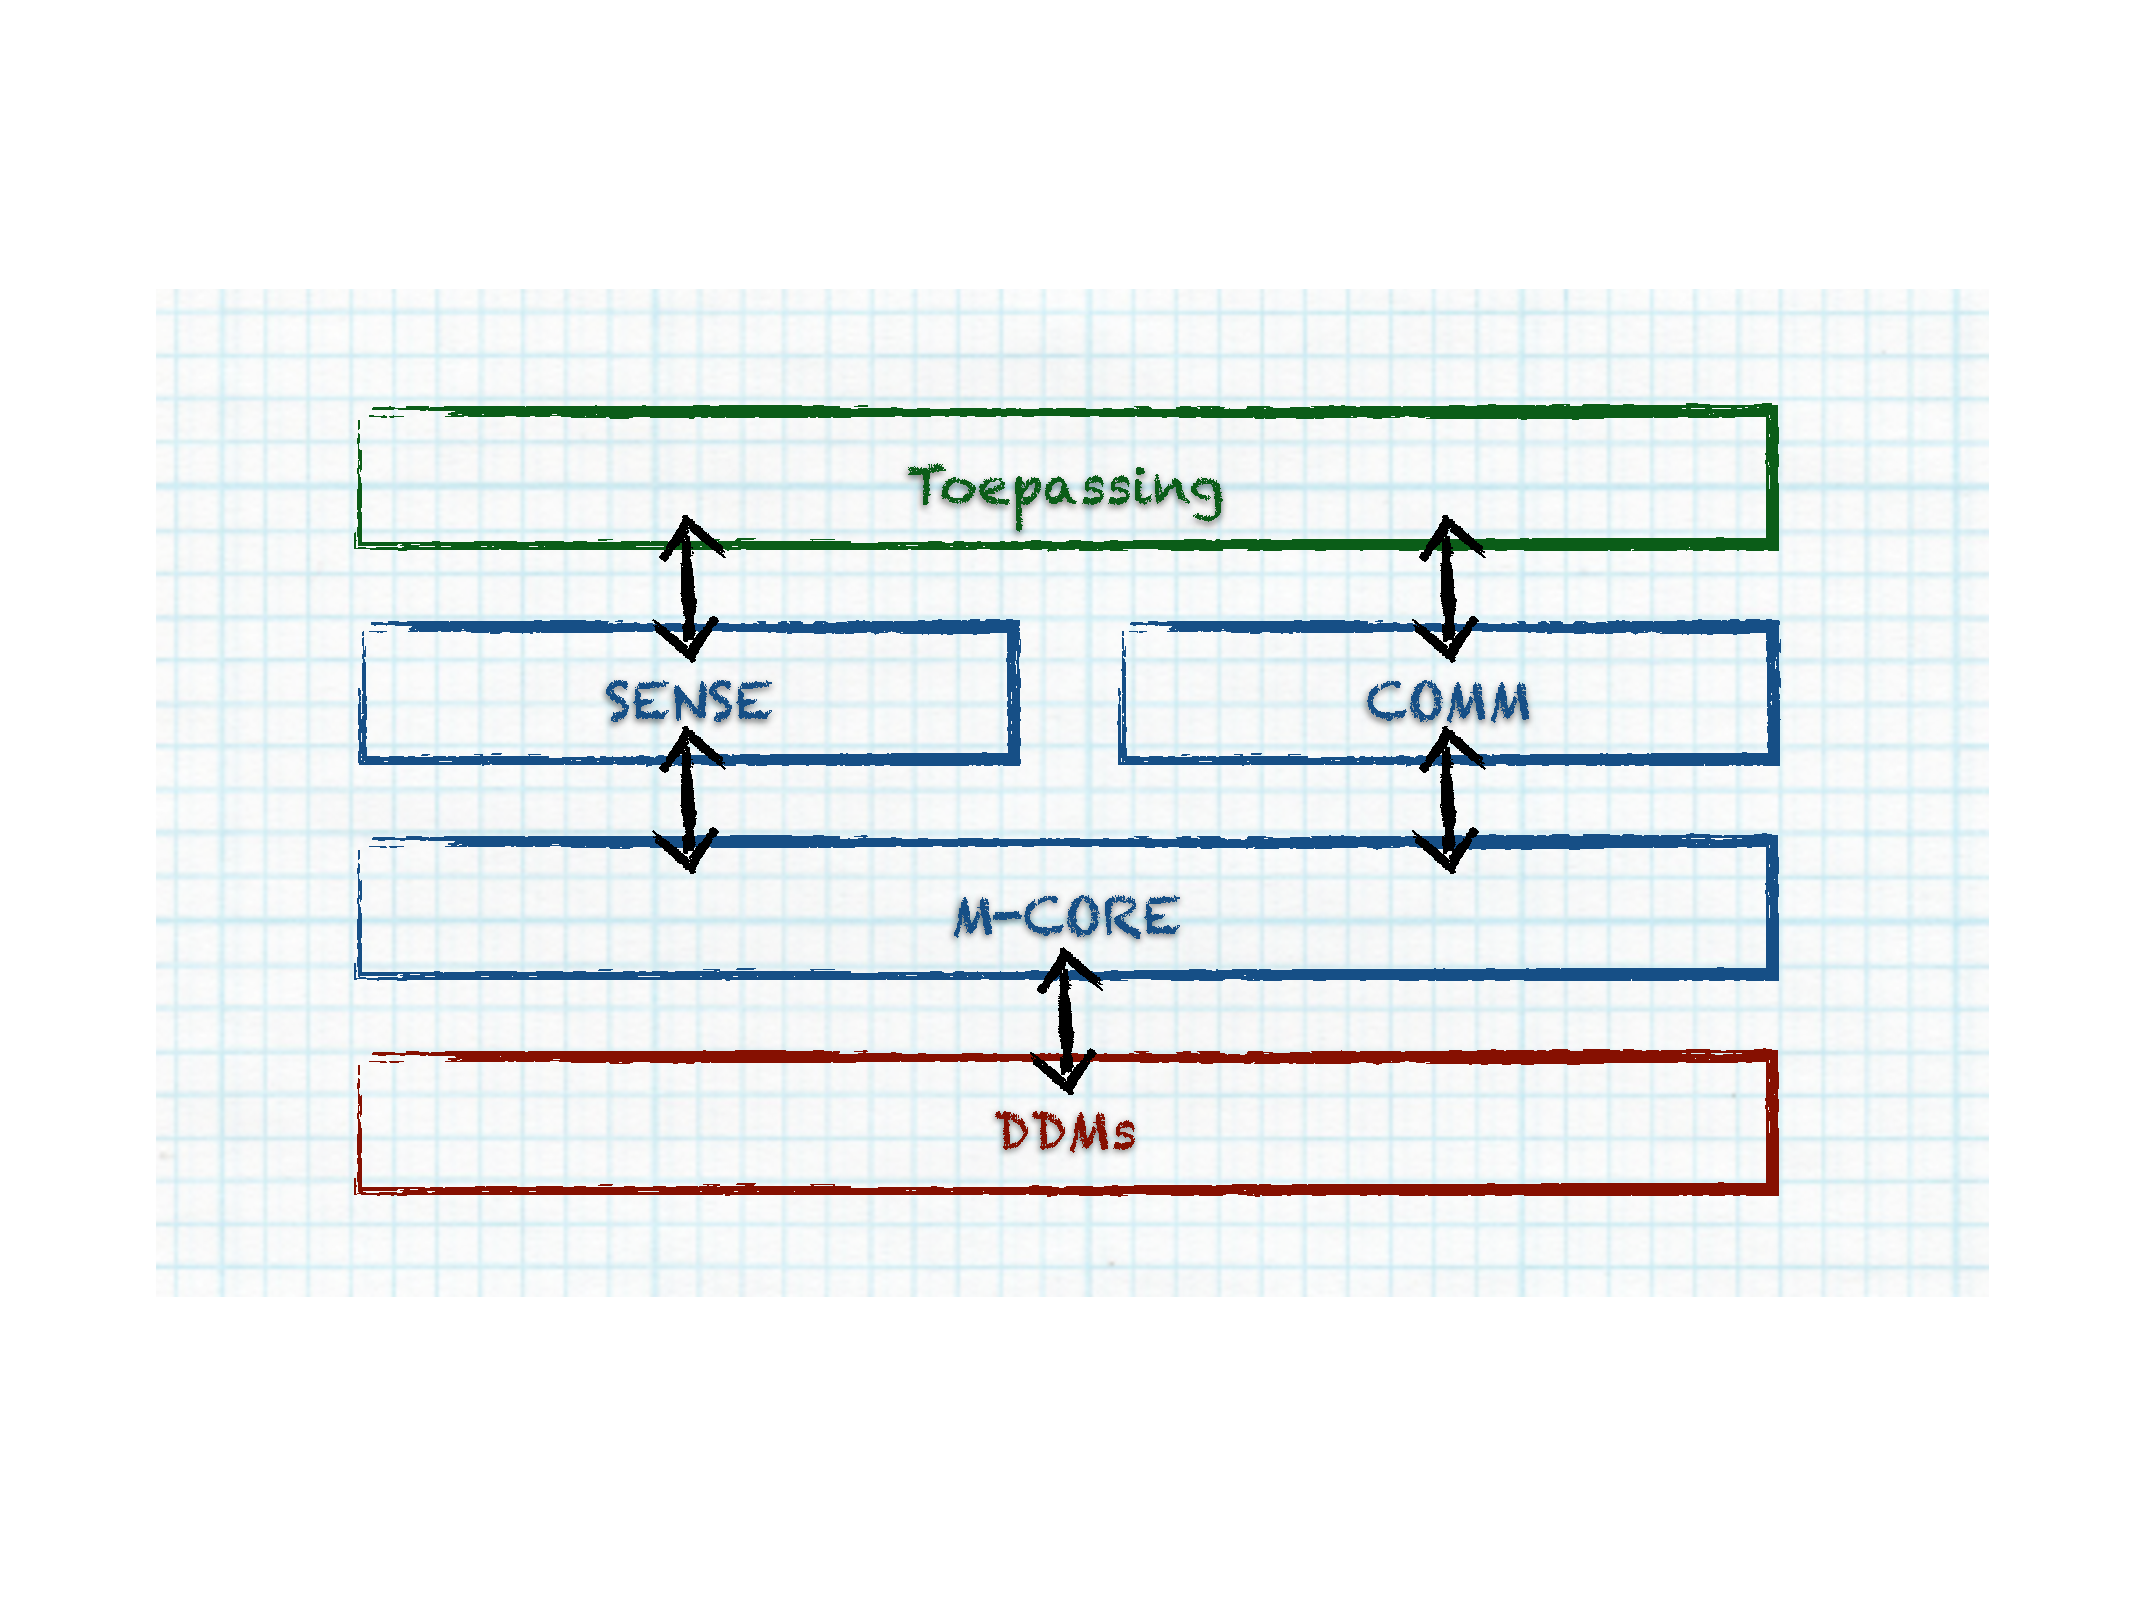
\includegraphics[width=\linewidth]{resources/di-sec-architecture.pdf}
  \caption{Architectuur van Di-Sec. \citep{valero2012di}}
  \label{fig:di-sec-architecture}
\end{figure}

De drie modules vormen als het ware een API voor de DDMs en de manier waarop de
COMM en Sense modules de toegang tot alle in- en uitvoer, zowel de
netwerkcommunicatie als de toegang tot de sensoren, hermetisch afsluiten, toont
aan dat Di-Sec op zich reeds een raamwerk is voor het ontwikkelen van
sensorknopen.

Naast dit raamwerk, biedt Di-Sec tevens een eigen DSL aan om Di-Sec te
gebruiken: de M-Core controle taal (MCL). Deze laat toe om met een beperkte
taal de nodige sjablonen te maken waarmee nieuwe modules kunnen ontwikkeld
worden en om de nodige aanpassingen te doen aan de configuratiebestanden.

\subsubsection*{Architectuur voor een sensorknoop}
\label{subsubsection:node-architecture}

Daar waar Di-Sec zich vooral focust op het aanbieden van een API voor het
ontwikkelen van detectie modules, gaat \citep{zhang2000intrusion} een stap
verder en verrijkt de architectuur van een sensorknoop met verschillende
modules, gericht op de onderliggende processen van een IDS. Zo worden
beveiligde communicatiemodules voorzien, is er een co\"operatieve detectie
module en voorzien zij globaal aggregerende modules om tot een consensus te
komen op het niveau van het netwerk. Deze architectuur is schematisch
weergegeven in figuur \ref{fig:node-architecture}.

\begin{figure}[ht]
  \centering
  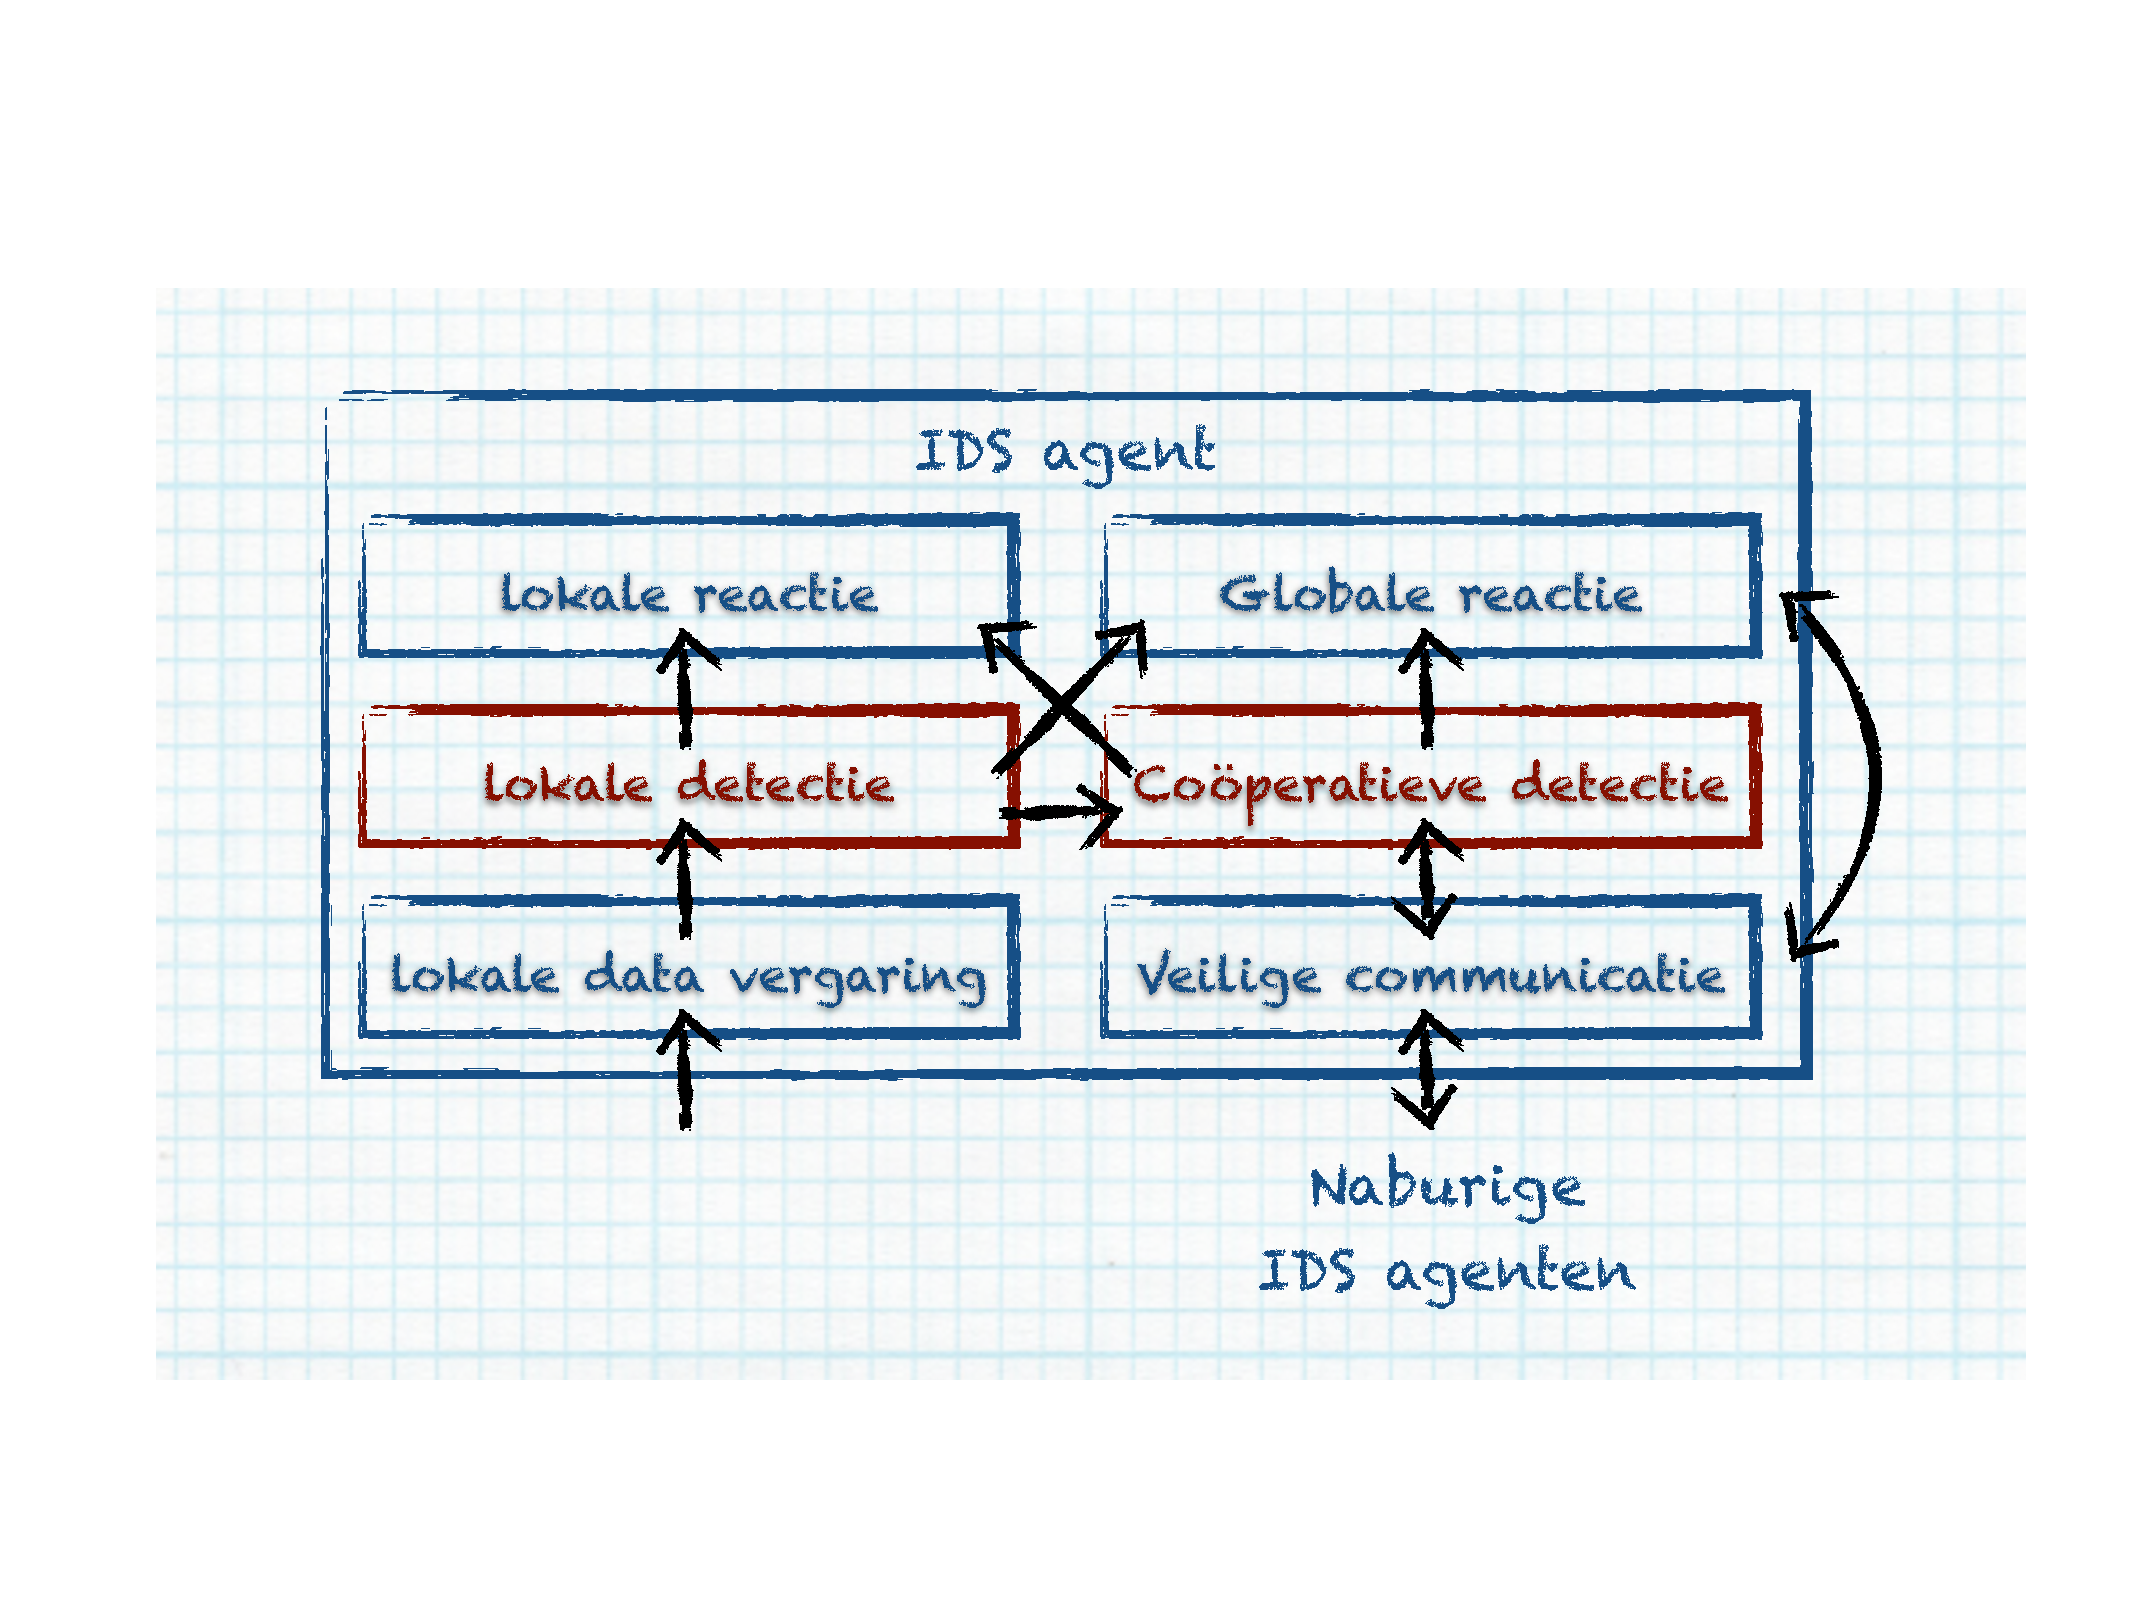
\includegraphics[width=0.5\linewidth]{resources/node-architecture.pdf}
  \caption{Conceptueel model voor een IDS op een sensorknoop. \citep{zhang2000intrusion}}
  \label{fig:node-architecture}
\end{figure}

De co\"operatieve modules voorzien bv. mogelijkheden om zekerheden te koppelen
aan beweringen over bepaalde gebeurtenissen. Op deze manier biedt de
architectuur een zeer specifiek aanbod aan functionaliteit specifiek voor het
bouwen van een IDS.

Een gelijkaardige architectuur wordt voorgesteld in \citep{krontiris2008lidea}.
LIDeA is een uitgewerkte architectuur voor de idee\"en die reeds aan bod kwamen
in sectie \ref{subsection:cooperation} en vormen het platform waarop het
co\"operatieve algoritme van \citep{krontiris2009cooperative} ge\"end is. Figuur
\ref{fig:lidea-architecture} toont de LIDeA architectuur.

\begin{figure}[ht]
  \centering
  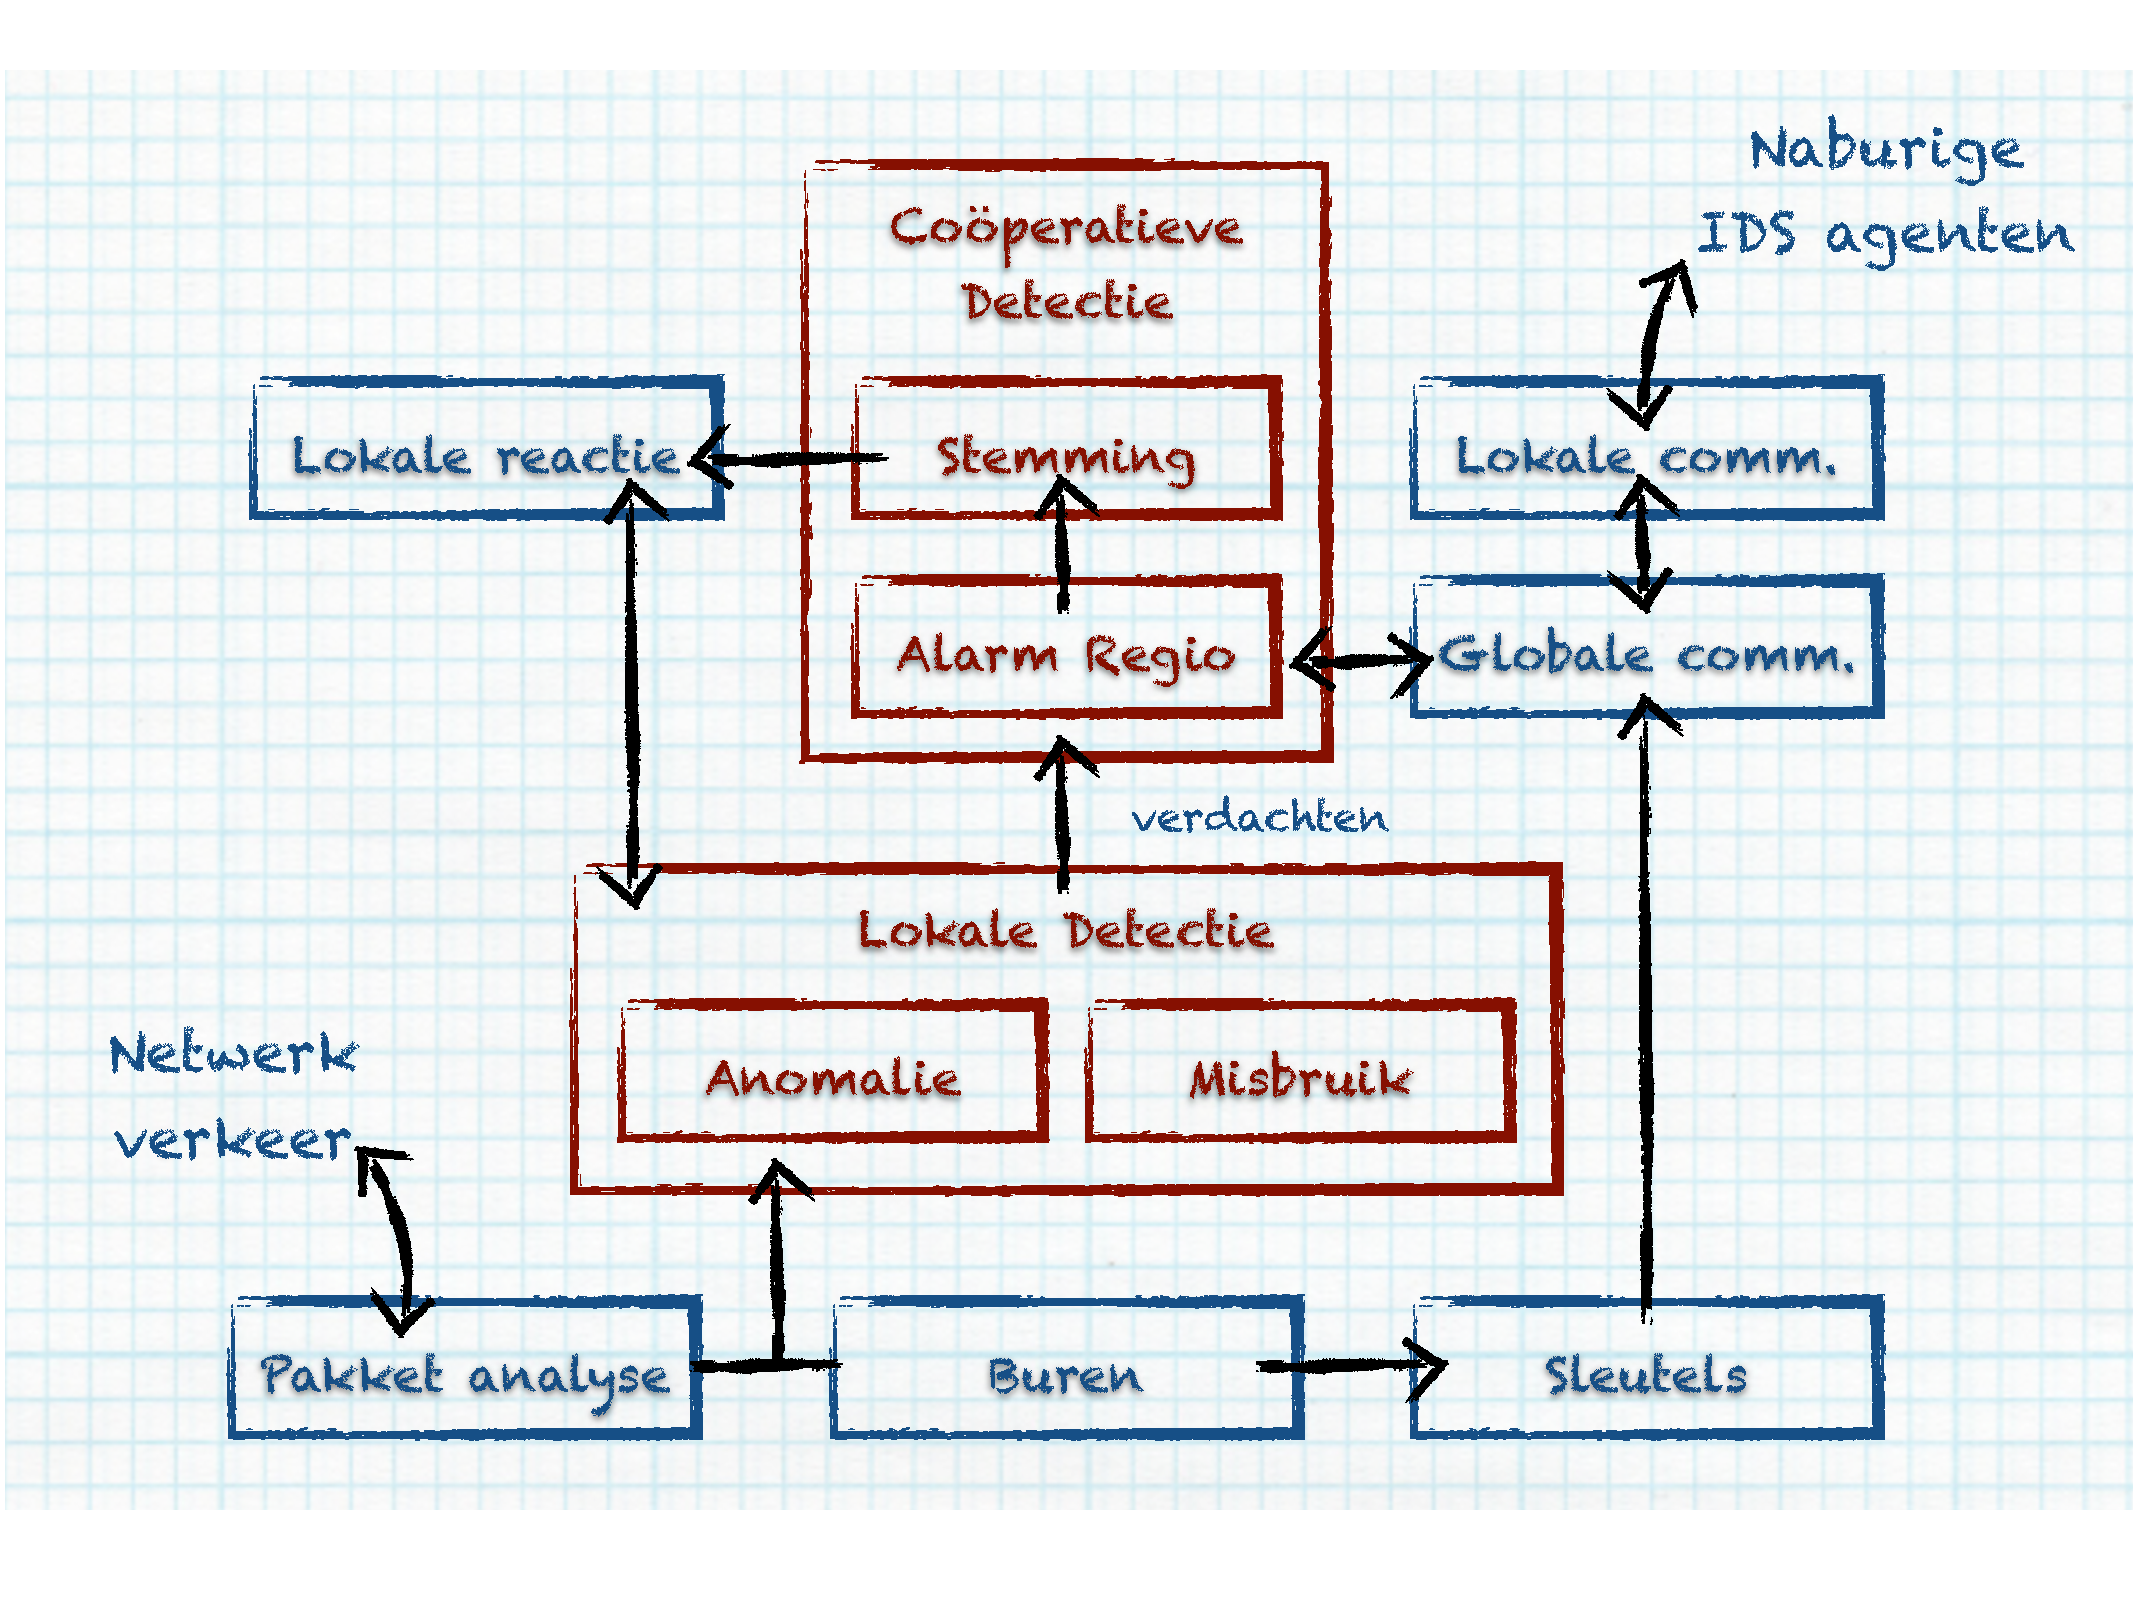
\includegraphics[width=0.5\linewidth]{resources/lidea-architecture.pdf}
  \caption{Architectuur van LIDeA. \citep{krontiris2008lidea}}
  \label{fig:lidea-architecture}
\end{figure}
